%-----------------------------------------------------
%  Introduction
%-----------------------------------------------------

\section{서론}
\subsection{연구 동기}

페로브스카이트(Perovskite) 구조를 가지고 있는 결정에 레이저를 쏘았을 때 Figure \ref{fig:waveguide} 에서 볼 수 있듯이 빛이 결정의 바깥쪽으로 퍼지는 현상을 관찰할 수 있었고, wave guiding effect에 의한 현상으로 추정하였다. Wave guiding effect\는 굴절률 차이에 의한 경로 변경이나 에너지 출입의 메커니즘에 의해서 빛이 특정 장소로 모이는 현상을 뜻한다. Yarita (2017)의 연구와 같이 페로브스카이트의 구조, 광학적 특성을 분석한 실험에서는 XRD(X-ray diffraction), TRPL(Time-Resolved Photoluminescence), PL(Photoluminescence)등 여러가지 장비를 통해 분석을 하였지만 중심으로부터 가장자리까지의 경향성을 분석하는 것은 없었다 \cite{yarita2017dynamics}. 특히 PL 분석에서는 PL로 찍었을 때 나오는 개형의 half width\과 peak에 대해서만 분석하였지만 wave guiding effect의 명확한 원인은 찾지 못하였다. 본 논문에서는 그 원인을 명확히 파악하고자 PL data\를 exciton peak과 biexciton peak에 대해서 따로 분석해보고자 하였다. 

\begin{figure}[H]
	\begin{center}
			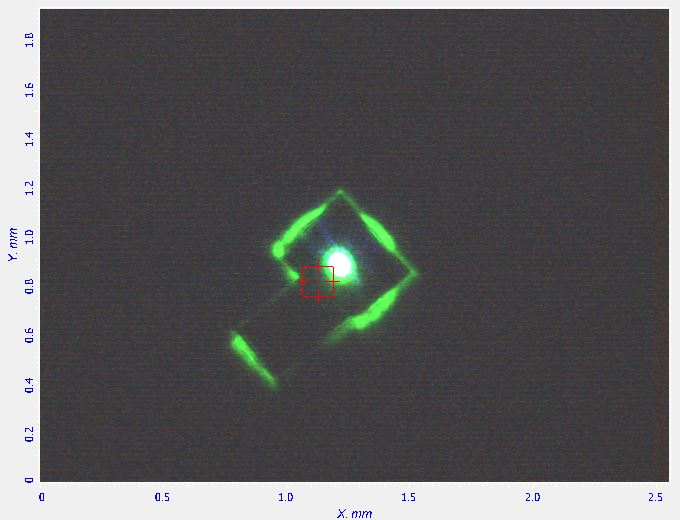
\includegraphics[width=0.6\textwidth]{waveguiding_effect}
	\end{center}
	\caption{Appearance of $\rm CsPbBr3$ single crystal when laser is shot on it.}
	\label{fig:waveguide}  
\end{figure}

\subsection{이론적 배경}

\subsubsection{Perovskite}
Green et al.(2014)에 의하면 페로브스카이트는 L. A. Perovski의 이름을 따서 명명된 물질로, 처음 발견된 $\rm CaTiO_3$  같은 구조를 가진 결정을 통틀어서 부르는 말이다. 일반적으로 $\rm ABX_3$로 쓰며, Figure 2와 같은 결정구조를 가지고 있다. 여기서 A와 M에는 여러 금속 양이온들이 해당되고, X에는 보통 16족, 17족 음이온들이 해당된다.


\begin{figure}[H]
	\begin{center}
			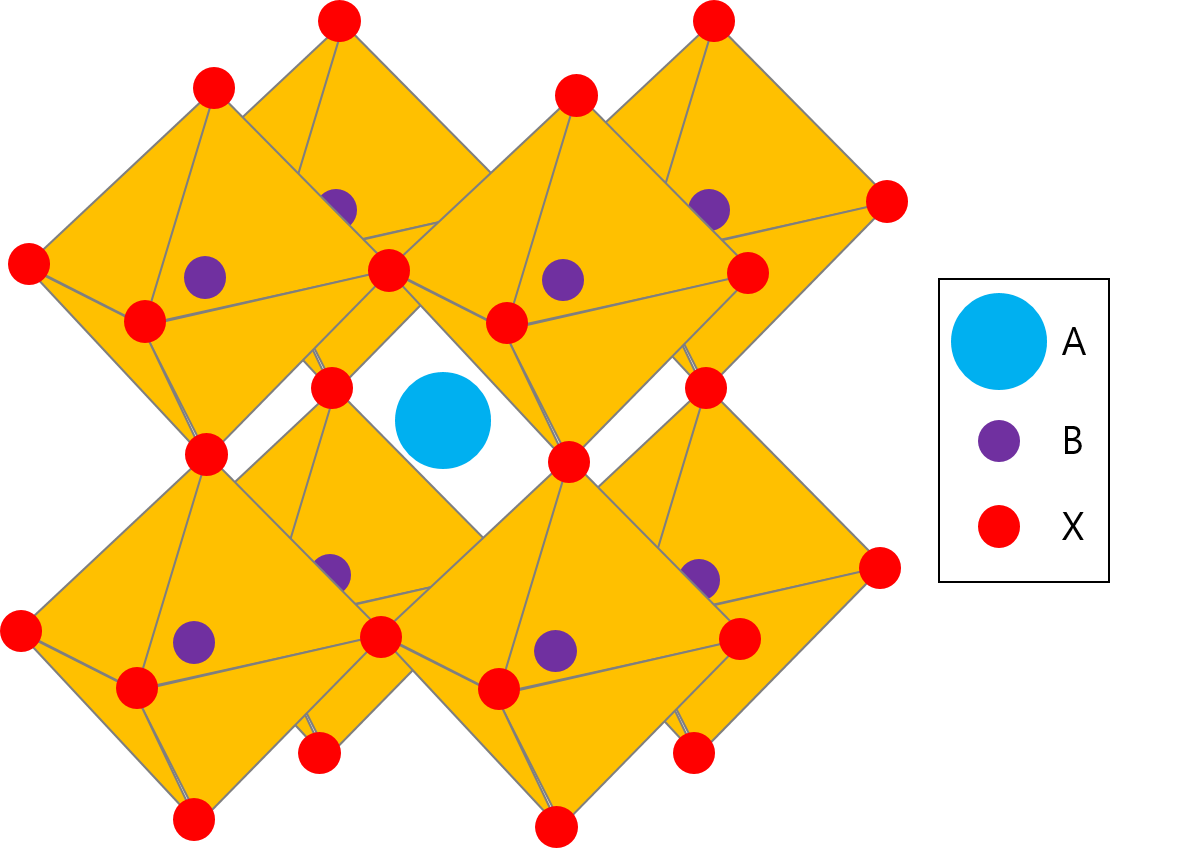
\includegraphics[width=0.6\textwidth]{perovskite}
	\end{center}
	\caption{Basic structure of perovskite.}
	\label{fig:perov} 
\end{figure}

A위치에는 금속뿐만 아니라 유기물인  methylammonium $\rm(CH_3NH_3^+)$이나 ethylammonium $\rm(CH_3CH_2NH_3^+)$를 넣어 페로브스카이트를 구성할 수 있다. Green et al.(2014)에 의하면 쇼트키-퀘이서 효율 한계(Shockley Queisser Efficiency Limit)에 의해 물질의 밴드갭에 따라 전지 효율의 이론적 최댓값이 존재한다\cite{green2014emergence}. 페로브스카이트는 각 자리에 여러 물질을 바꿔 넣을 수 있으므로 이론적인 최대 효율값에 비슷하게 도달할 수  있는 장점이 있다. 이 뿐만 아니라 가능한 밴드갭 영역이 넓고 꼭짓점을 공유하는 팔면체들의 회로망 덕분에 캐리어의 이동성이 좋아서 전하가 잘 수송되기도 한다\cite{green2014emergence}.

또, 페로브스카이트는 합성이 간편하며 태양빛을 잘 흡수하기 때문에 각광받고 있으며, 이와 관련되어 여러 연구가 진행되고 있다. Huang(2009)\은 페로브스카이트에 defect가 존재하여 물성을 탐색할 때 정확하지 못하다는 문제를 해결하기 위해서 단결정을 제작하기도 하였다\cite{huang2009fabrication}. 본 연구에서는 단결정을 제작하는 새로운 방식 중 하나인 PDMS(Polydimethylsiloxane) stamping을 이용하여 단결정을 제작하였다.
\\

\subsubsection{Photoluminescence}

\begin{figure}[H]
	\begin{center}
			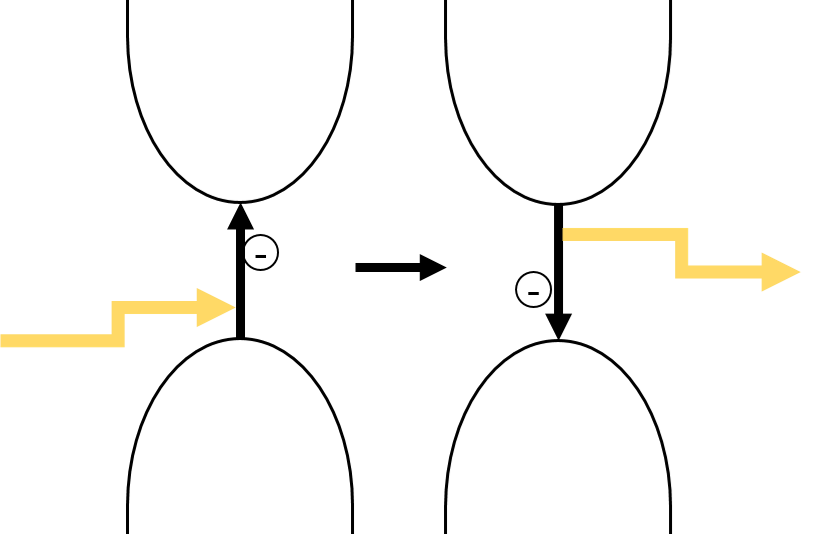
\includegraphics[width=0.8\textwidth]{PL}
	\end{center}
	\caption{Energy released from the relaxation process of excited electrons.}
	\label{fig:pl} 
\end{figure}

PL\는 광자를 통해 에너지를 흡수한 물질이 그 에너지를 다시 방출하는 것을 이르는 것이다. 이론적으로는 넣어준 빛의 파장과 동일한 파장의 빛이 나올 수도 있지만 보통은 에너지가 더 낮은, 파장이 더 긴 빛이 방출되게 된다. 

빛이 방출되는 과정은 크게 photoexcitation, relaxation, radiative recombination의 세 가지 과정으로 나뉜다. photoexcitation은 외부에서 주어진 빛에 의해 전자가 들뜨는 현상을 이르는 것이고 relaxation은 들뜬 전자가 전도띠에서 에너지가 가장 낮은 부분으로, 정공이 원자띠에서 에너지가 가장 높은 부분으로 이동하는 과정이다. 마지막으로 radiative recombination 과정은 들뜬 전자가 다시 정공과 결합하는 과정을 의미한다(Figure \ref{fig:pl}를 참고). 이때 방출되는 빛의 파장 별 intensity를 PL로 측정하여 data\를 얻을 수 있다.
\\

\subsubsection{Exciton, biexciton의 의미}
\begin{figure}[H]
	\begin{center}
			
\includegraphics[width=0.6\textwidth]{exciton_biexciton}
	\end{center}
	\caption{image of exciton and biexciton.}
	\label{fig:ex}  
\end{figure}
Exciton은 앞서 말한 PL에서의 측정 과정에서 양공과 전자 하나의 쌍을 말하며, 이 것이 두개가 쌍을 이루고 있을 때 그것을 biexciton이라 칭한다(Figure \ref{fig:ex} 참고). Triexciton 또한 존재하지만 그 존재 빈도가 극히 적어서 스펙트럼에 나타나지 않는다. 
\\
\subsubsection{Waveguiding effect}
Waveguiding effect란 도파관 효과로, 빛이나 에너지가 여러가지 이유에 의해서 특정 지점으로 모이거나 빛의 경로가 조절되는 현상을 말한다. 가장 기본적인 예시로 빛이 전반사되는 광섬유가 있다. J.Valenta (2002), Jin (1999)\와 같이 광결정에서 에너지의 이득을 보기 위해서 발생하는 waveguiding effect가 있기도 하다\cite{valenta2002waveguiding} \cite{jin1999band}. 


\subsubsection{ND filter}
ND(Neutral Density) filter\는 특정한 파장대의 빛을 투과시키면 세기가 감소하는 특성을 가지고 있다. 이는 강한 레이저 빛이 광학기구에 직접 닿으면 센서나 광학 기구가 손상될 수 있기 때문에 사용한다. 투과율 T는 OD(Optical Density)값으로 정의되며 편의에 의해 OD값에 따라 ND filter 표기는 식 \ref{eq:002}\와 같이 결정된다.
\begin{equation}
T(\%)~=~10^{-OD}~\times~100
\label{eq:002}
\end{equation}
\\

\subsection{선행연구 및 한계}
본 연구에 앞서 수행한 연구에서는 XRD, TRPL, PL을 통해 단결정 페로브스카이트의 구조적, 광학적 특성을 분석하였다. XRD는 성공적이었으나 위치별로 분석한 PL 분석에서는 스펙트럼이 비대칭적으로 나타났음에도 불구하고 peak와 half width로만 분석했기에 경향성을 분석할 때에 exciton peak 와 biexciton peak의 합의 경향성을 볼 수 있었다. 하지만 결정 내부의 radiative recombination에서 방출되는 빛의 defect와 결정의 순도에 관한 것은 두 가지 peak을 따로 분석해야 알 수 있다. Chen(2018)은 exciton과 biexciton을 따로 생각하고 온도에 따른 exciton과 biexciton peak의 변화를 분석하였고, 본 연구에서는 이를 참고하였다 \cite{chen2018room}. 
\\

\subsection{연구 목적 및 연구 문제}
본 연구는 PL 분석시에 나타나는 peak의 exciton, biexciton별 분석을 통하여 wave guiding effect의 원인을 분석하는 것이 목적이다. wave guiding effect\와 전자의 photoluminescence\와의 연관성을 찾기 위해 위치에 따른 exciton, biexciton peak의 intensity를 조사하고 경향성을 분석한다.

본 연구에서 제시하는 연구 문제는 다음과 같다:
\begin{enumerate}
	\item $\rm CsPbBr_3$ 단결정에 레이저를 쏘았을 때 바깥쪽에서 그 빛이 나타나는 것은 wave guiding effect에 의한 것인가?
	\item Wave guiding effect에 의한 효과라면 전자의 photoluminescence와는 어떤 관련이 있는가? 
\end{enumerate}

